\section{Fit and Compare Models}
\subsection{Business Series}
Since the Business series is found to be non-stationary,differencing is applied before a model is fitted. A first difference is taken to remove the trend identified previously.
\begin{figure}[H]
    \centering
    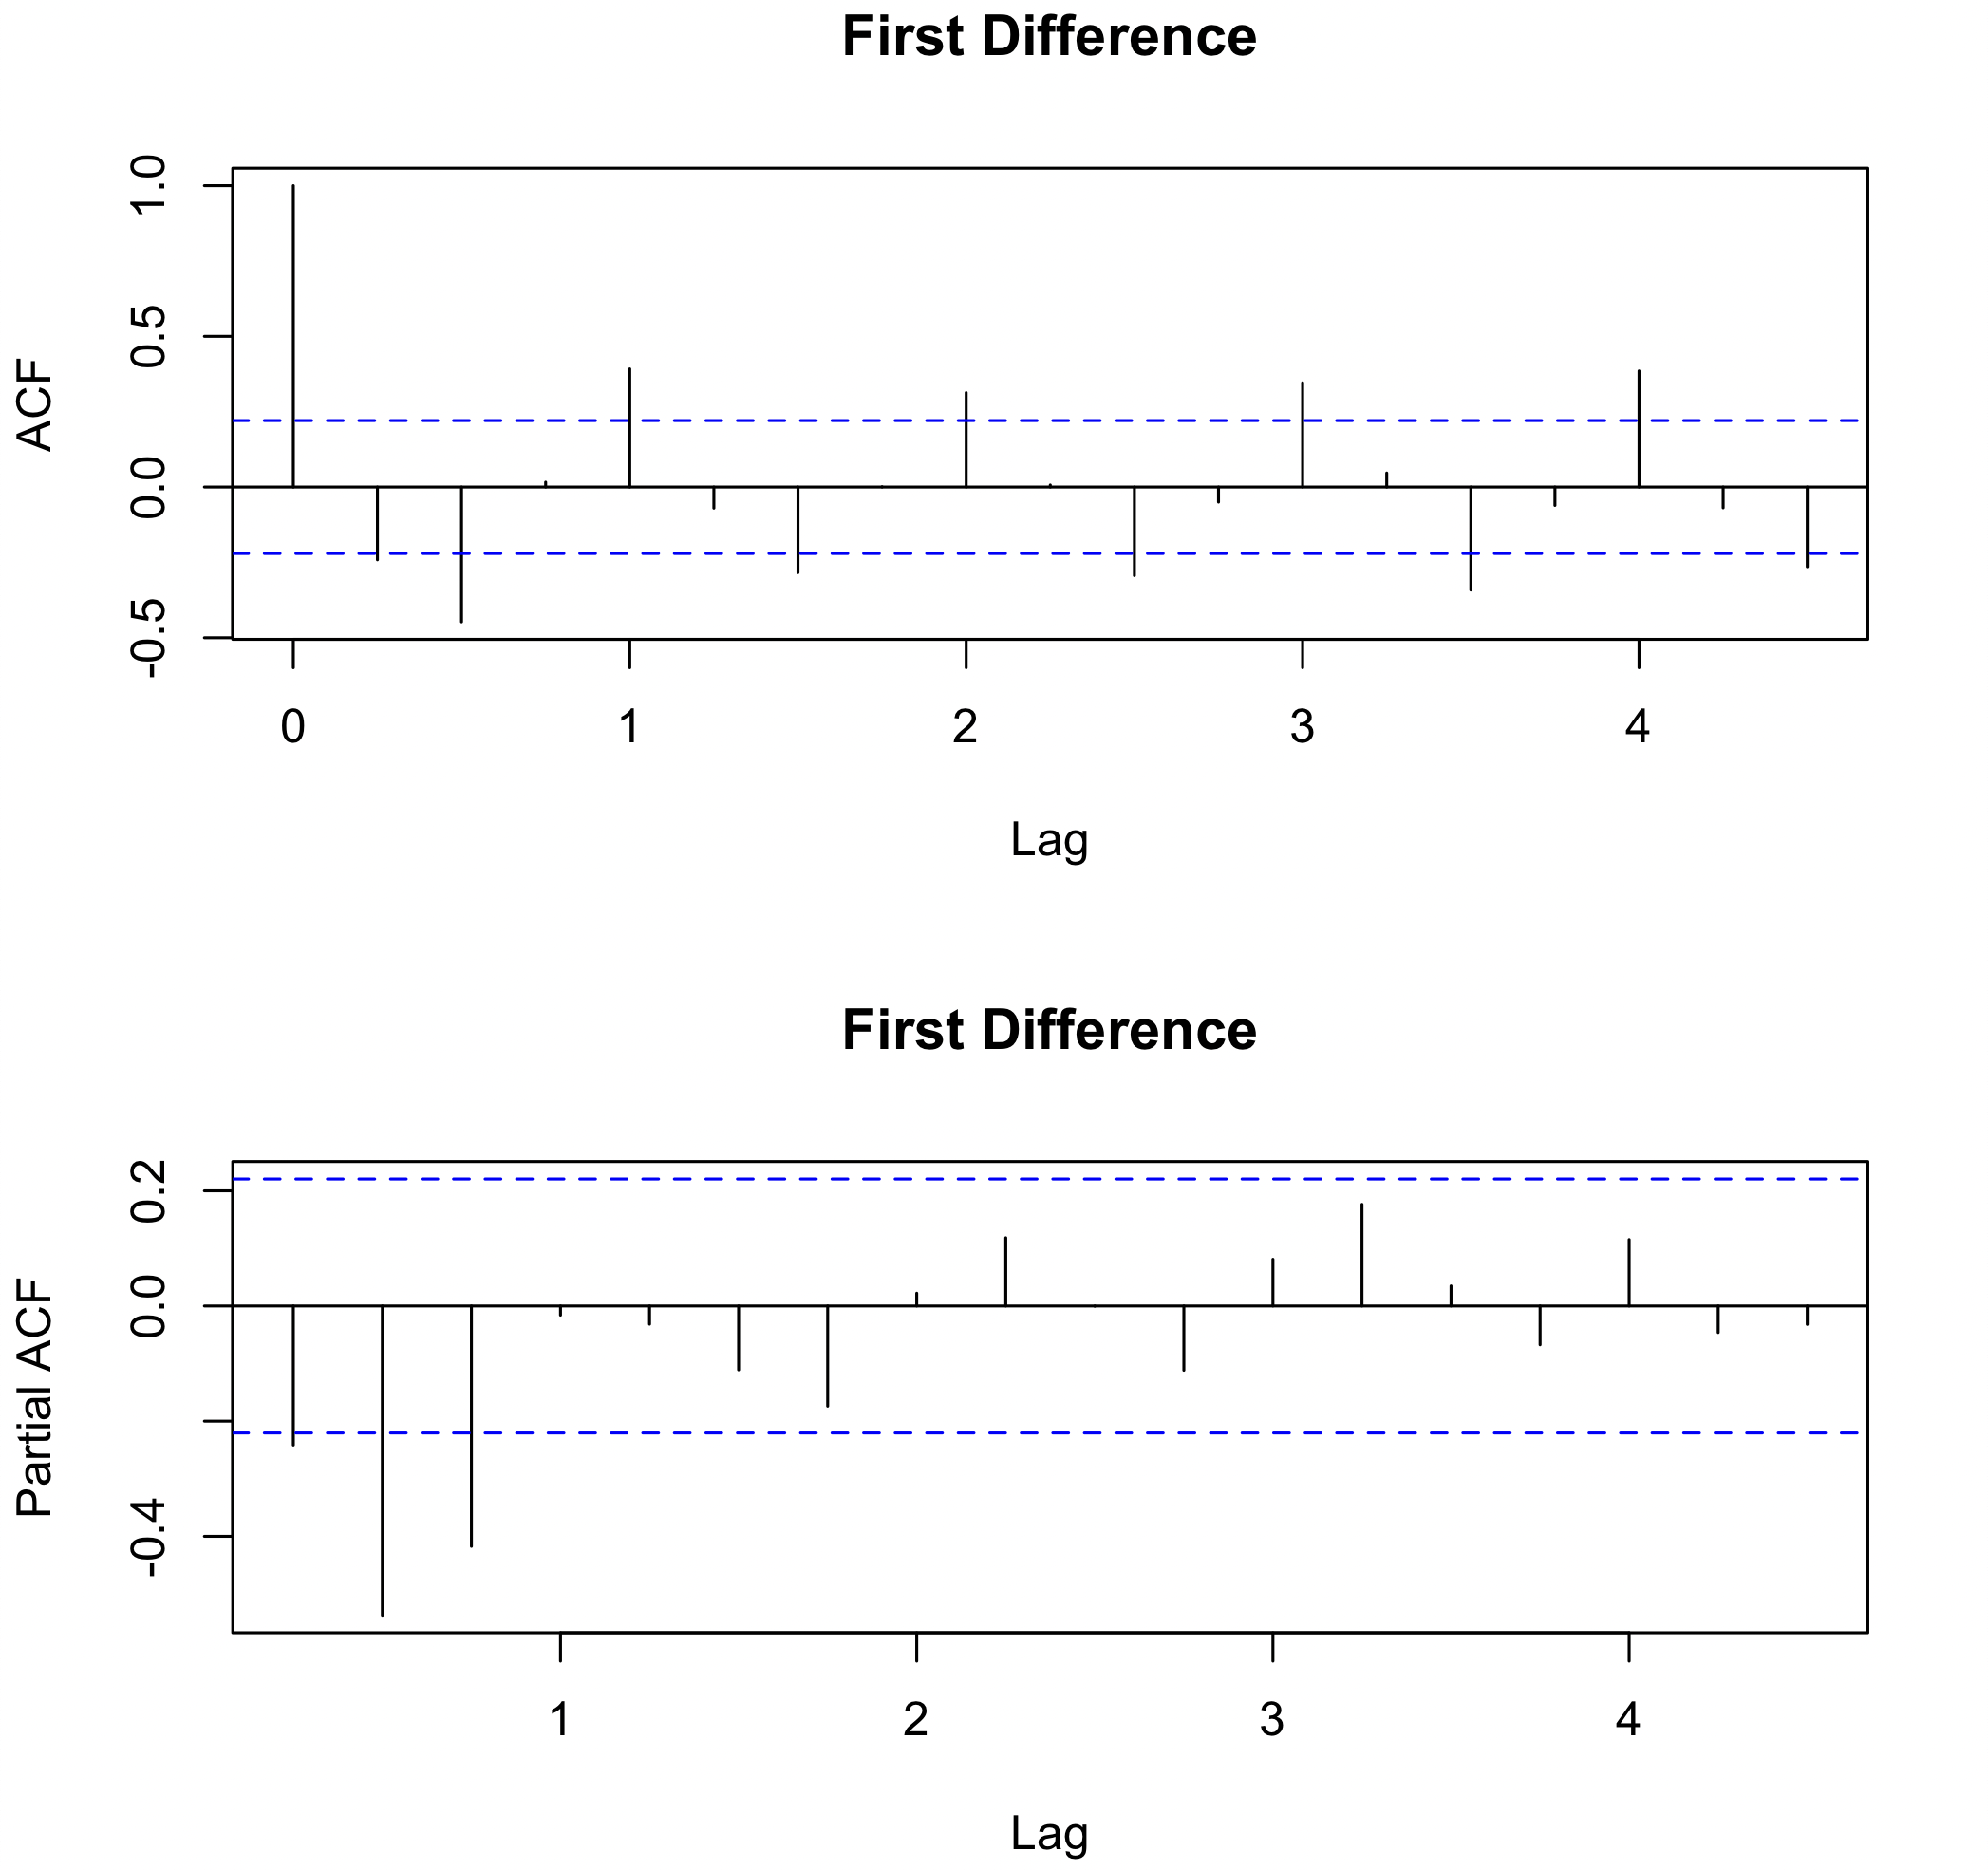
\includegraphics[width=0.5\linewidth]{fig/y1diff.png}
\end{figure}
\vspace{-0.4cm}
\noindent The correlogram of the first difference still shows a repeating pattern of significant autocorrelations, and the seasonal component identified has not been removed.\\
A seasonal difference at lag 4 is therefore applied to the already first-differenced series.
\begin{figure}[H]
    \centering
    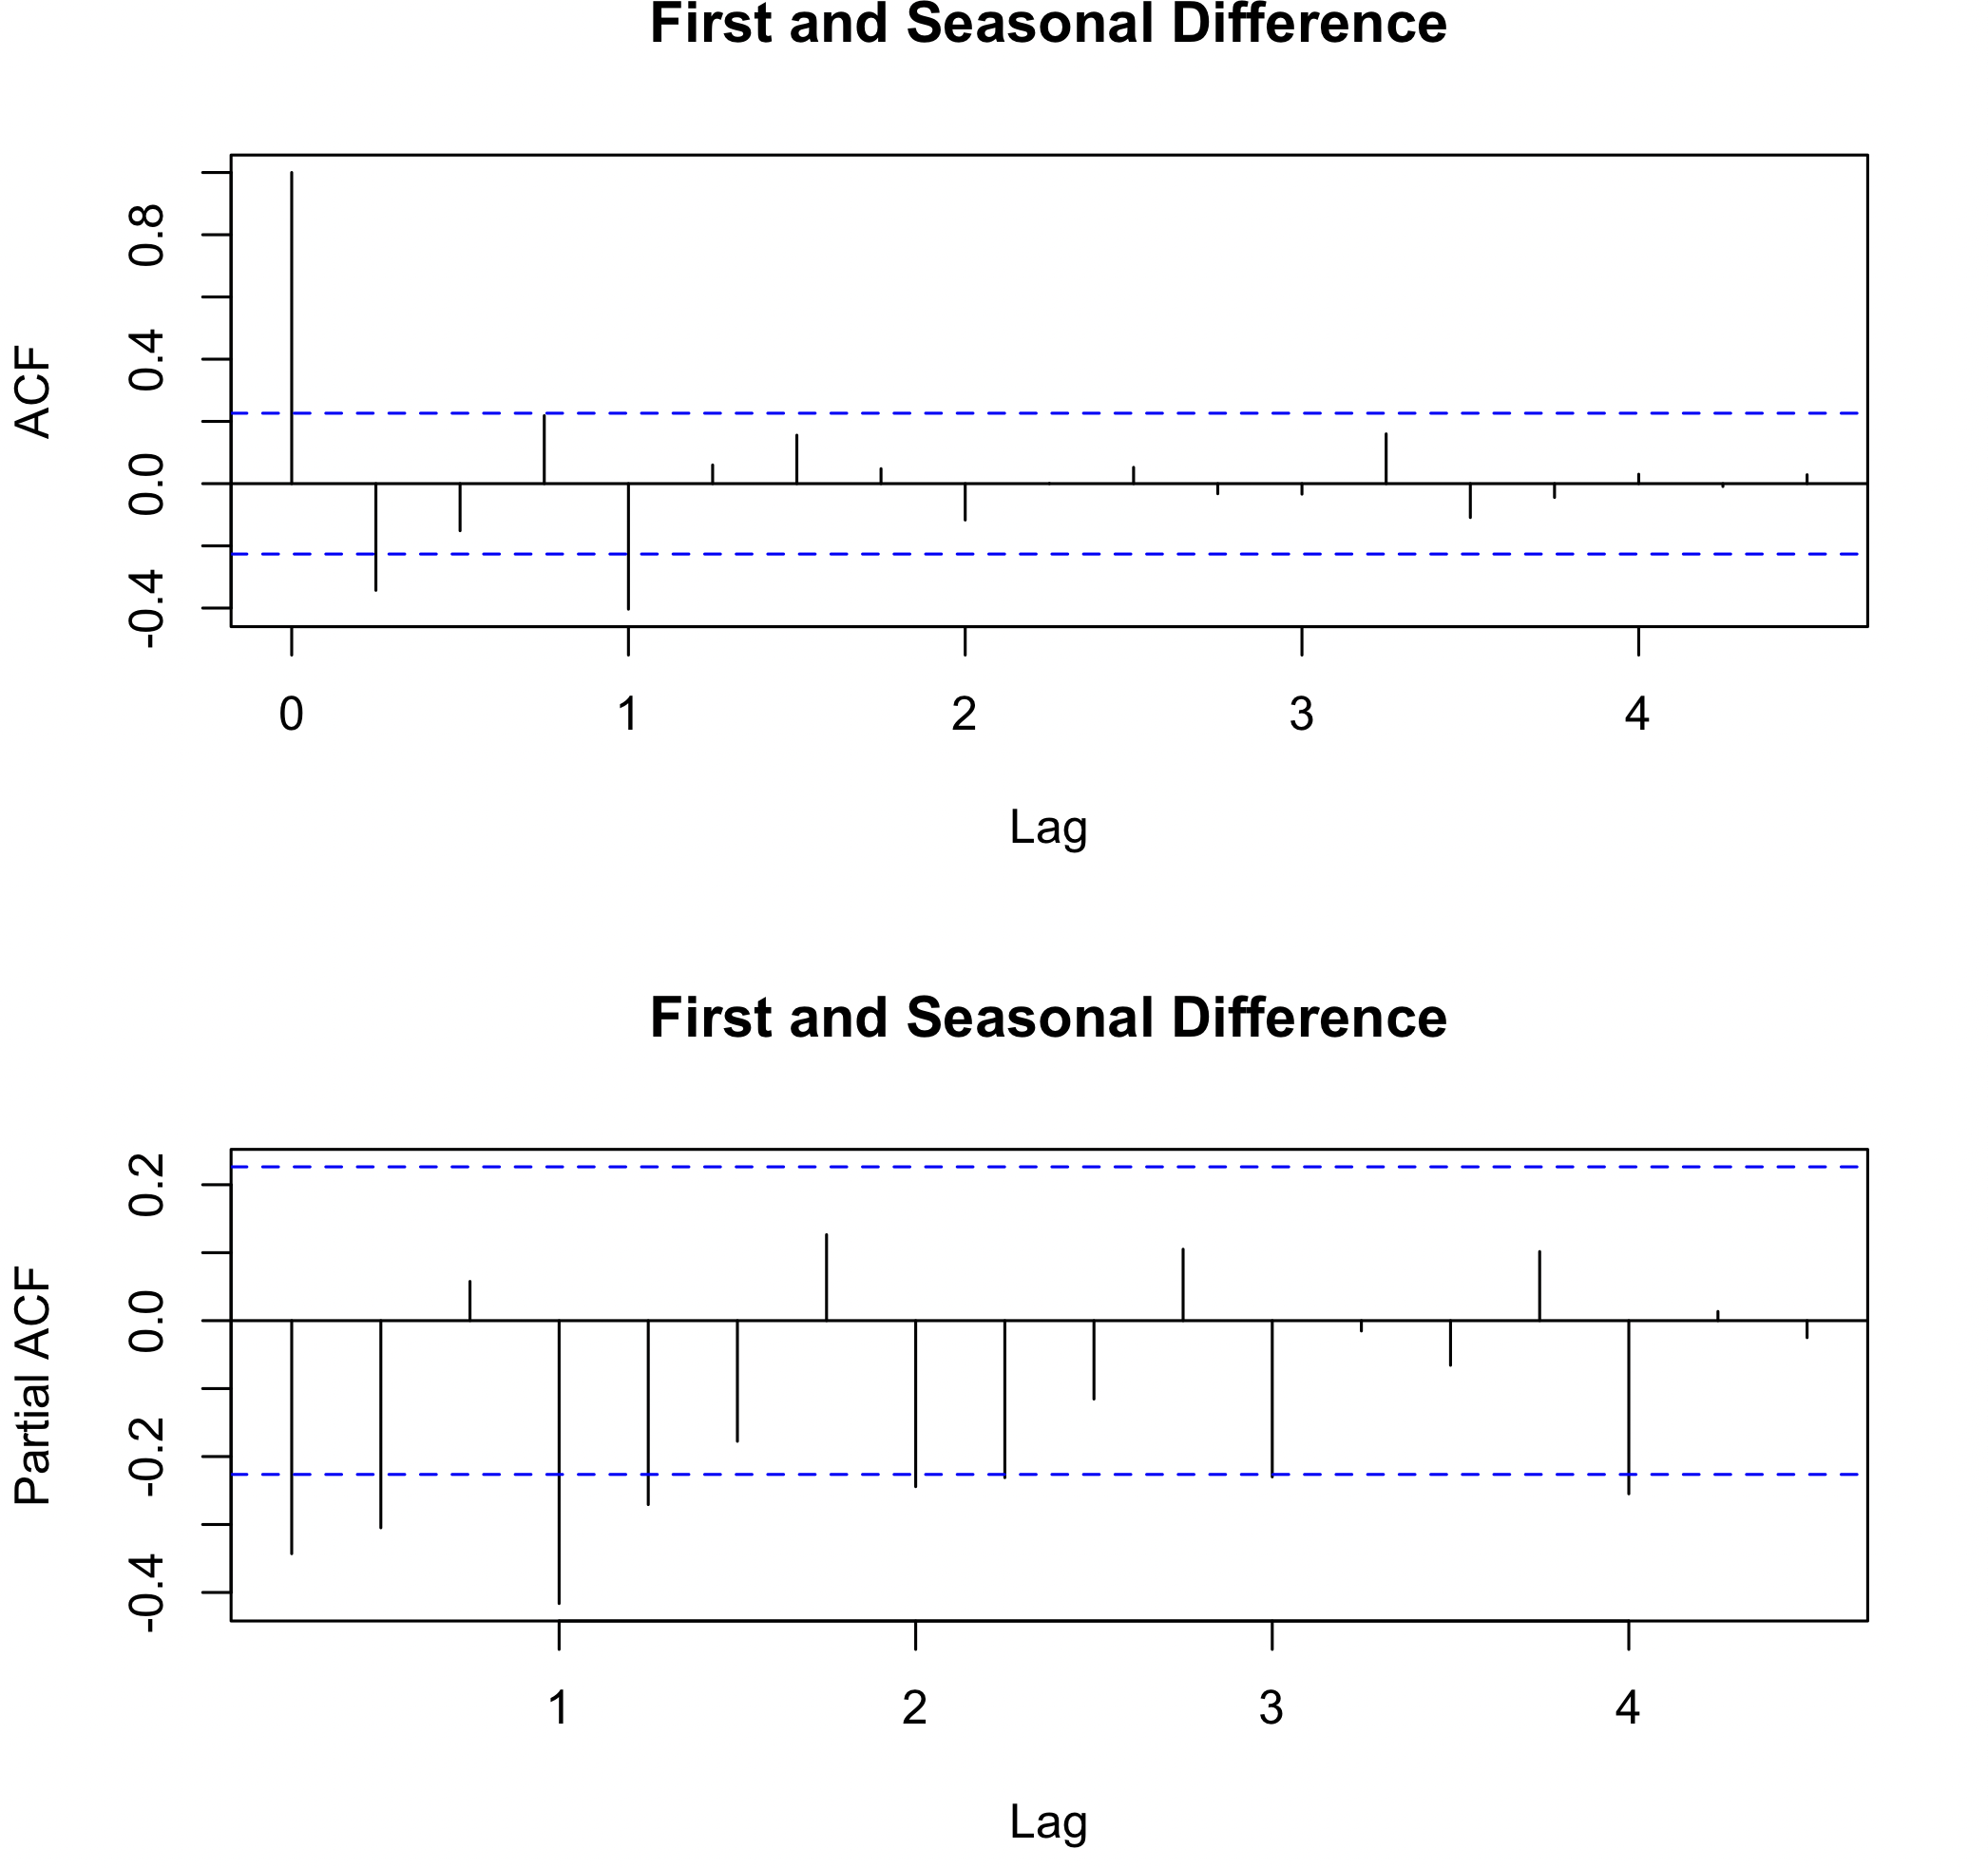
\includegraphics[width=0.5\linewidth]{fig/y1fsdiff.png}
\end{figure}
\noindent The correlogram now decays rapidly, with only a few significant lags and no remaining seasonal pattern, suggesting that d=1 and D=1 are appropriate differencing orders for the ARIMA search.\\
The \texttt{get.best.sarima} function defined in Lecture Notes Ch.7 is then used to identify the optimal SARIMA model.
% \begin{lstlisting}[language=R,basicstyle=\ttfamily\footnotesize]
% get.best.sarima <- function(x.ts, maxord = c(1,1,1,1,1,1))
% {best.aic <- Inf
%   n <- length(x.ts)
%   for(p in 0:maxord[1])for(d in 0:maxord[2]) for(q in 0:maxord[3])
%   for(P in 0:maxord[4])for(D in 0:maxord[5]) for(Q in 0:maxord[6])
%   {fit <- arima(x.ts,order=c(p, d, q),
%                  seasonal=list(order = c(P, D, Q),frequency(x.ts)),
%                  method = "CSS")
%     fit.aic <- -2 * fit$loglik + (log(n) + 1) * length(fit$coef)
%     if (fit.aic < best.aic)
%     {best.aic   <- fit.aic
%       best.fit   <- fit
%       best.order <- c(p, d, q, P, D, Q)}}
%   list(best.aic, best.fit, best.order)}
% \end{lstlisting}
\noindent The function evaluates all model orders up to maxord and selects the one with the lowest CAIC.
% \begin{lstlisting}[language=R]
% y1.best <- get.best.sarima(y1, maxord = c(2,2,2,2,2,2))
% y1.best
% \end{lstlisting}
\vspace{-0.4cm}
\begin{figure}[H]
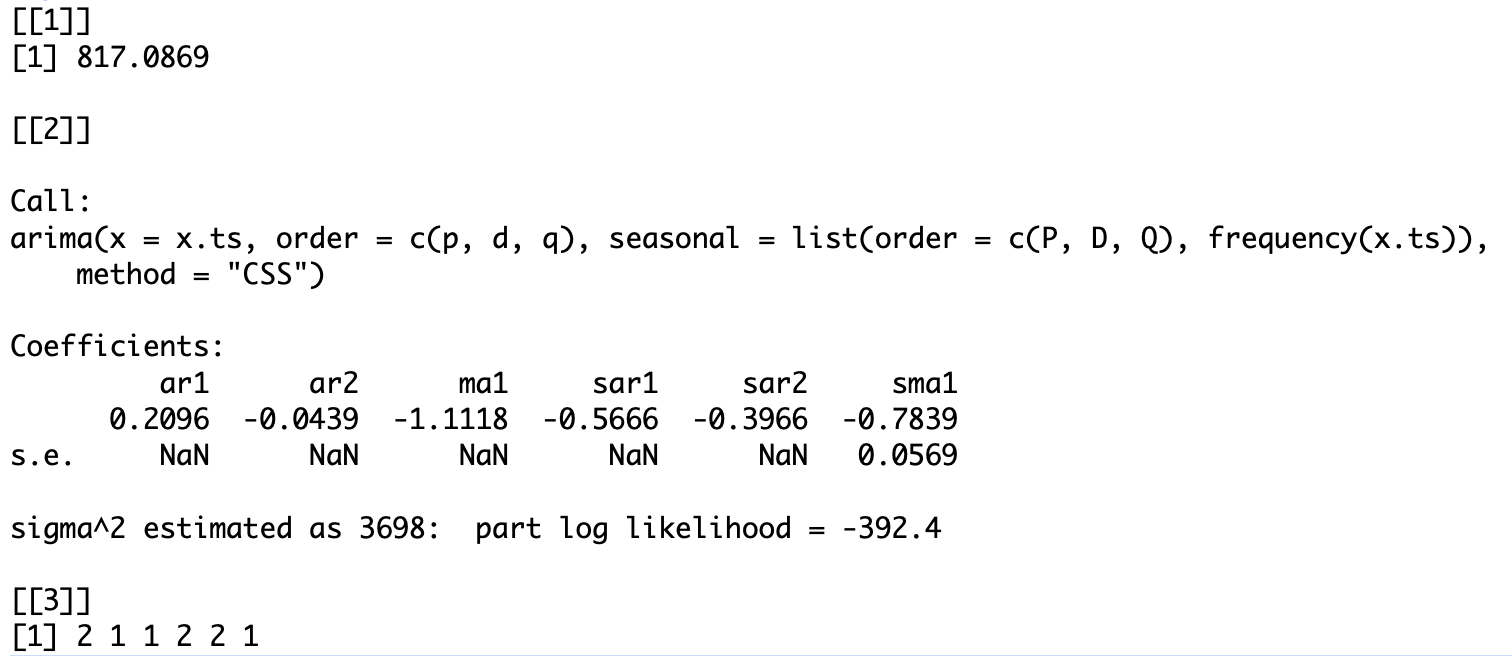
\includegraphics[width=0.75\linewidth]{fig/y1best.png}
\end{figure}
\vspace{-0.4cm}
\noindent Searching up to second order (\texttt{maxord = c(2,2,2,2,2,2)}) selects ARIMA$(2,1,1)(2,2,1)_4$ as the best fit. However, \texttt{confint()} cannot compute $95\%$ confidence intervals for most coefficients due to excessive seasonal differencing ($D=2$) relative to the small sample size ($n=80$). As the parameters are not reliably estimable, the model is not pursued further.
% \begin{lstlisting}[language=R]
% y1.best2 <- get.best.sarima(y1, maxord = c(2,1,2,2,1,2))
% y1.best2
% \end{lstlisting}
\vspace{-0.4cm}
\begin{figure}[H]
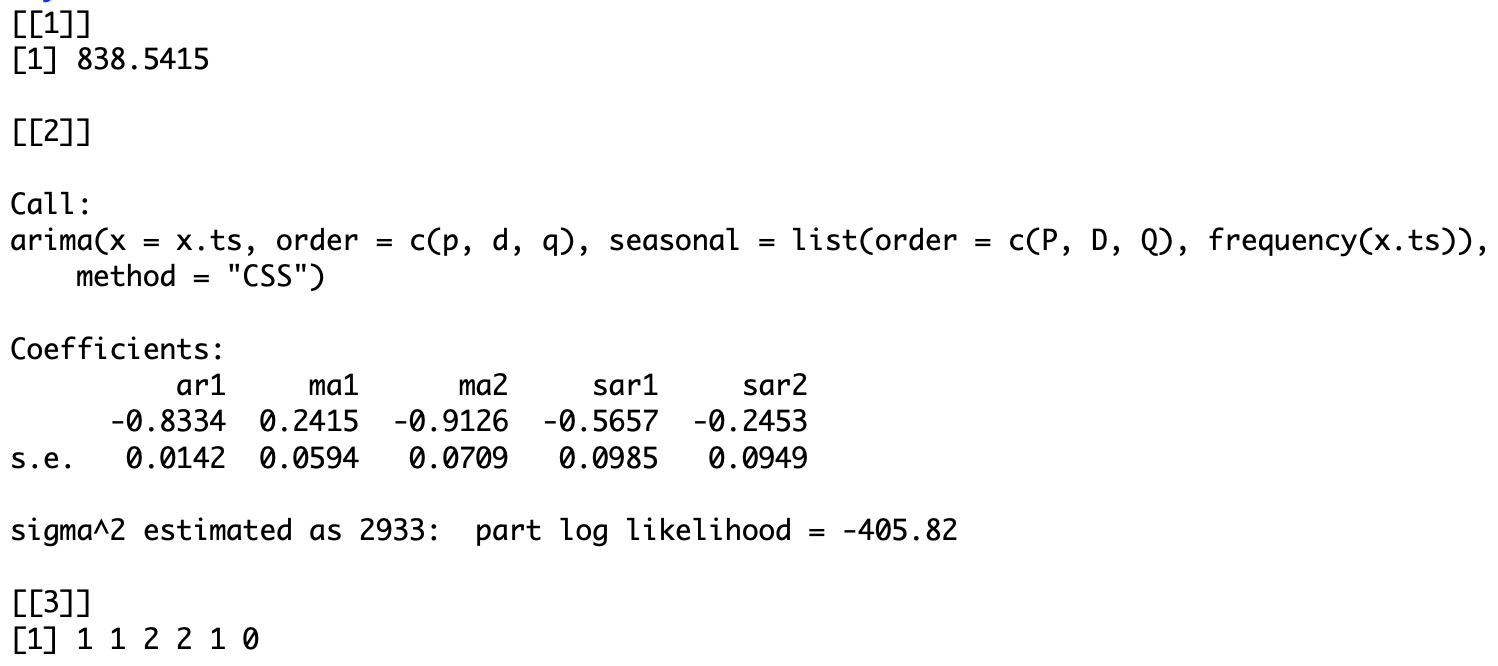
\includegraphics[width=0.75\linewidth]{fig/y1best2.png}
\end{figure}
\vspace{-0.4cm}
\noindent Restricting the search to at most one difference at each level ($d \leq 1$, $D \leq 1$), consistent with the differencing established above, identifies ARIMA$(1, 1, 2)(2, 1, 0)_4$ as the best-fitting model.
% \begin{lstlisting}[language=R]
% y1.sarima <- arima(y1, order = c(1,1,2),
%                 seasonal = list(order = c(2,1,0), 4),
%                 method = "CSS")
% y1.sarima
% \end{lstlisting}
\begin{figure}[H]
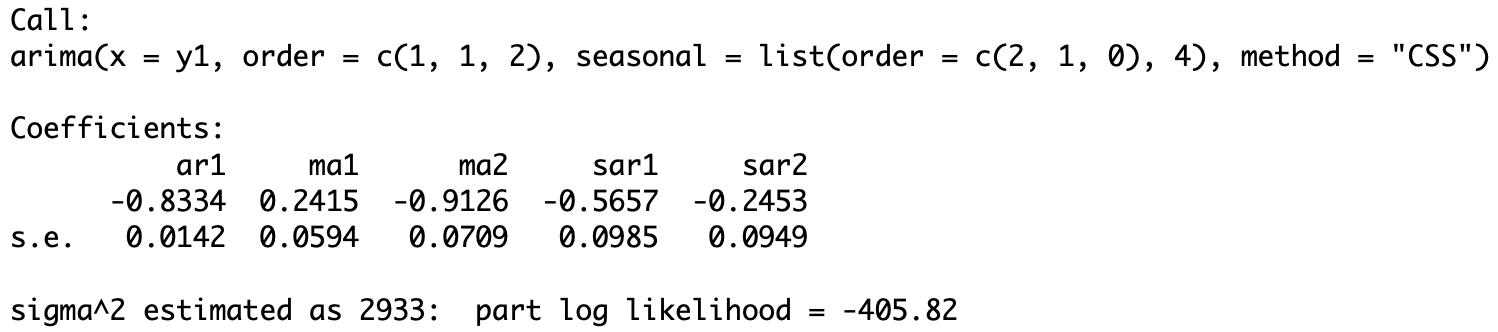
\includegraphics[width=0.75\linewidth]{fig/y1coef.png}
\end{figure}
\vspace{-0.4cm}
% \begin{lstlisting}
% confint(y1.safrima)
% \end{lstlisting}
\vspace{-0.4cm}
\begin{figure}[H]
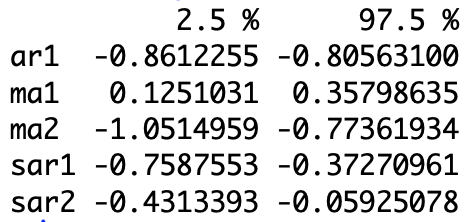
\includegraphics[width=0.25\linewidth]{fig/y1ci.png}
\end{figure}
\noindent All five coefficients are significantly different from zero, as none of the confidence intervals include zero; hence, no terms are removed. The fitted model with $\sigma^2 = 2933$ is
\vspace{-0.5cm}
\begin{align*}
x_t - x_{t-1} &= -0.8334(x_{t-1} - x_{t-2}) - 0.5657(x_{t-4} - x_{t-5}) - 0.2453(x_{t-8} - x_{t-9}) \\
&\quad + w_t + 0.2415w_{t-1} - 0.9126w_{t-2}.
\end{align*}
% \begin{lstlisting}[language=R]
% acf(resid(y1.sarima)^2, main="Squared Residuals")
% \end{lstlisting}
\vspace{-0.5cm}
\begin{figure}[H]
    \centering
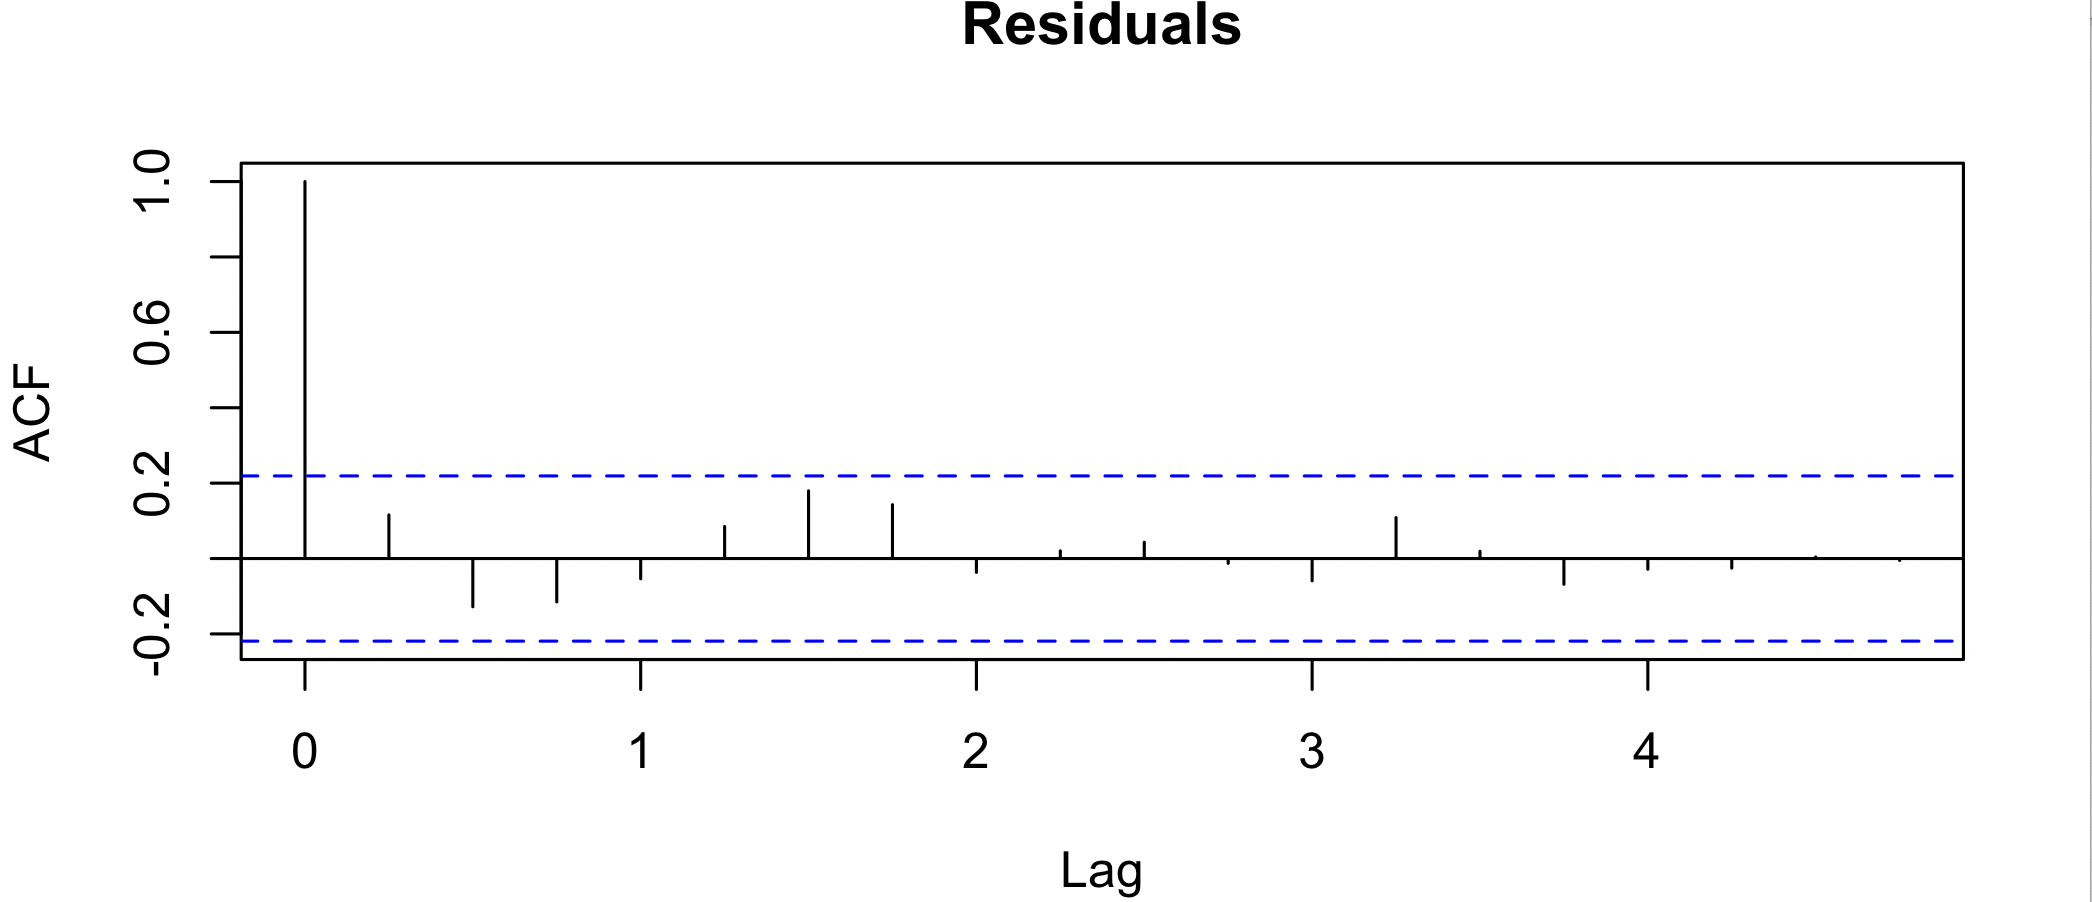
\includegraphics[width=0.75\linewidth]{fig/y1qr.png}
\end{figure}

\noindent The residual correlogram shows no significant autocorrelation, indicating white-noise behaviour and adequate model fit across trend and seasonality.
The \textbf{ARIMA$(1, 1, 2)(2, 1, 0)_4$} model is therefore selected as the final specification for the Business series.


\subsection{Holiday Series}

Since the Holiday series is found to be non-stationary, a first difference is applied before fitting the model to remove the trend identified previously.

\begin{figure}[H]
    \centering
    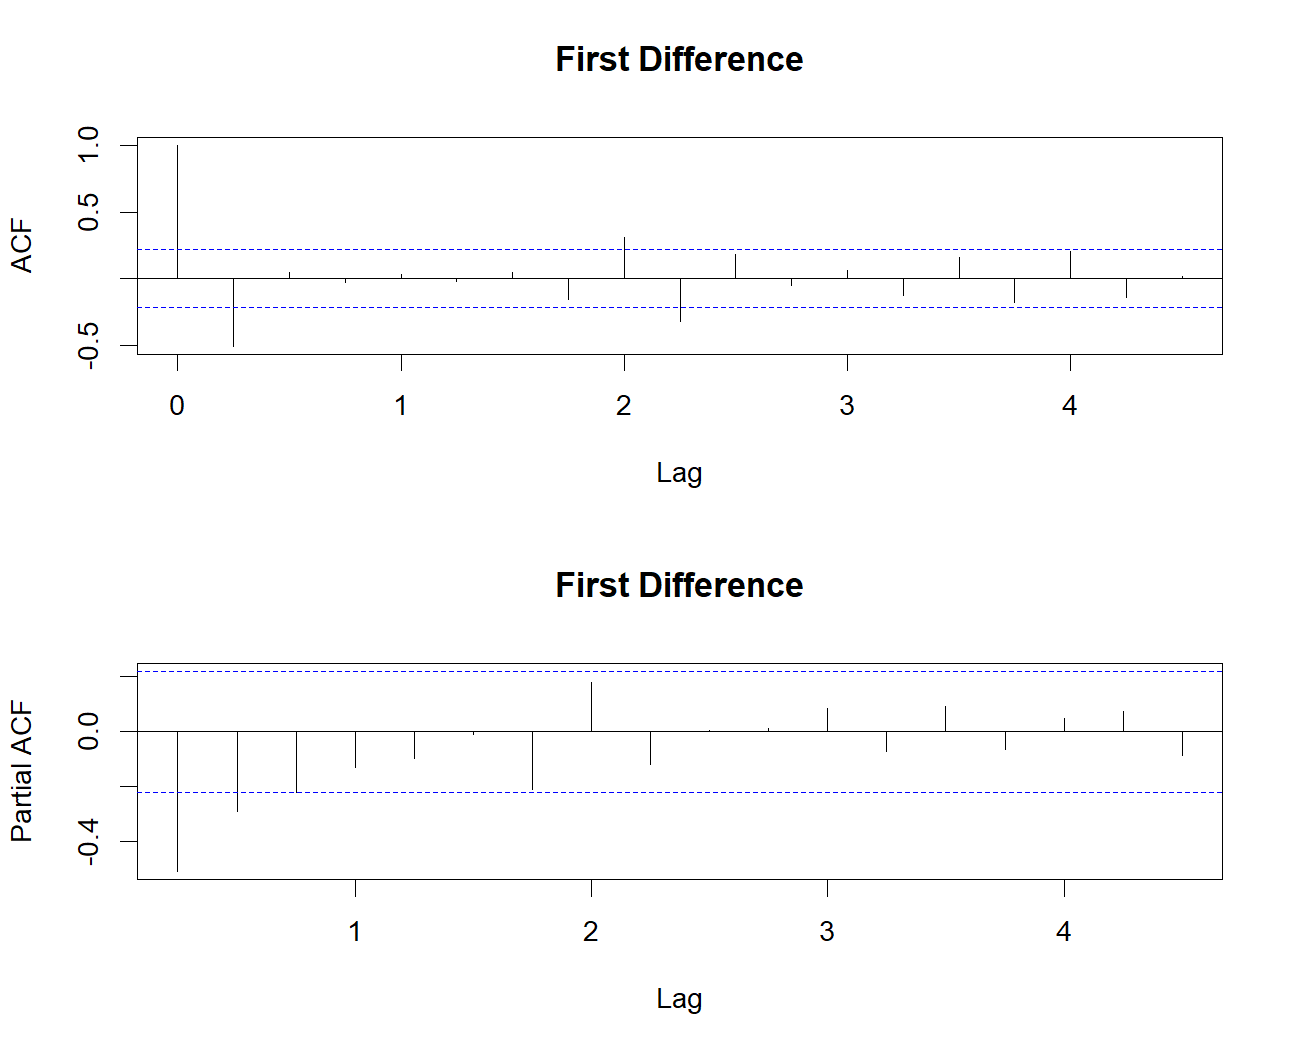
\includegraphics[width=0.75\linewidth]{fig/y2diff.png}
\end{figure}

\noindent The correlogram of the first-differenced series shows that the autocorrelations are substantially reduced, indicating that the trend has been largely removed. However, several significant autocorrelations remain at seasonal lags, suggesting that the seasonal component has not been completely removed. A seasonal difference at lag 4 is therefore applied to the first-differenced series.

\begin{figure}[H]
    \centering
    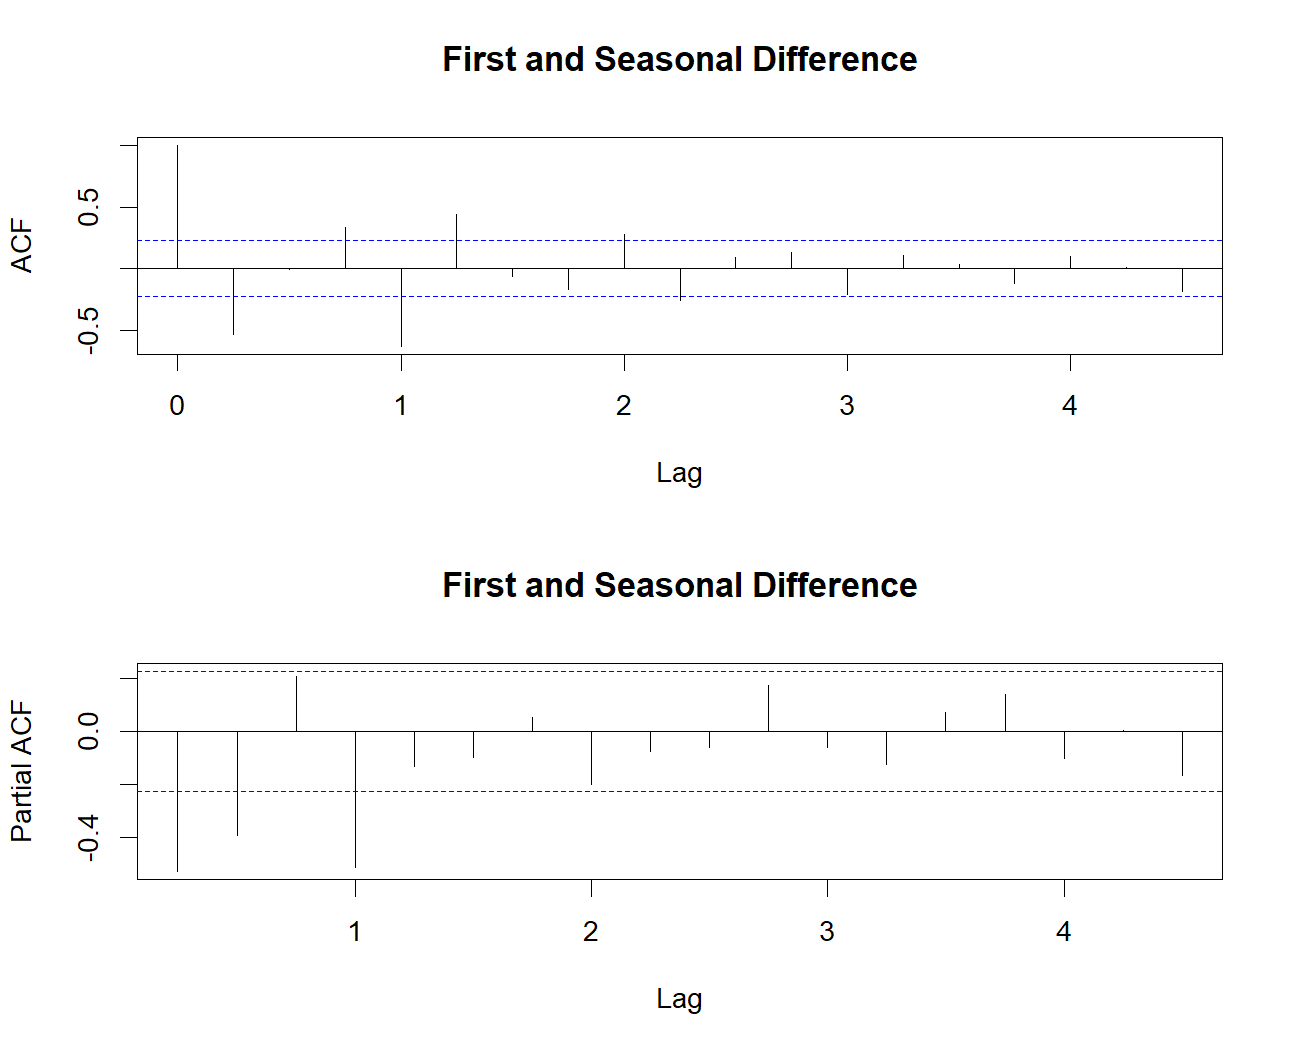
\includegraphics[width=0.75\linewidth]{fig/y2fsdiff.png}
\end{figure}

\noindent After applying both first and seasonal differencing, the autocorrelations decay more rapidly and the seasonal pattern is substantially reduced. Although some significant spikes remain, the differenced series is closer to stationarity. Therefore, \(d=1\) and \(D=1\) are considered appropriate starting values for the SARIMA model search.

\noindent The \texttt{get.best.sarima} function defined in Lecture Notes Ch.7 is then used to identify the optimal SARIMA model.


\begin{figure}[H]
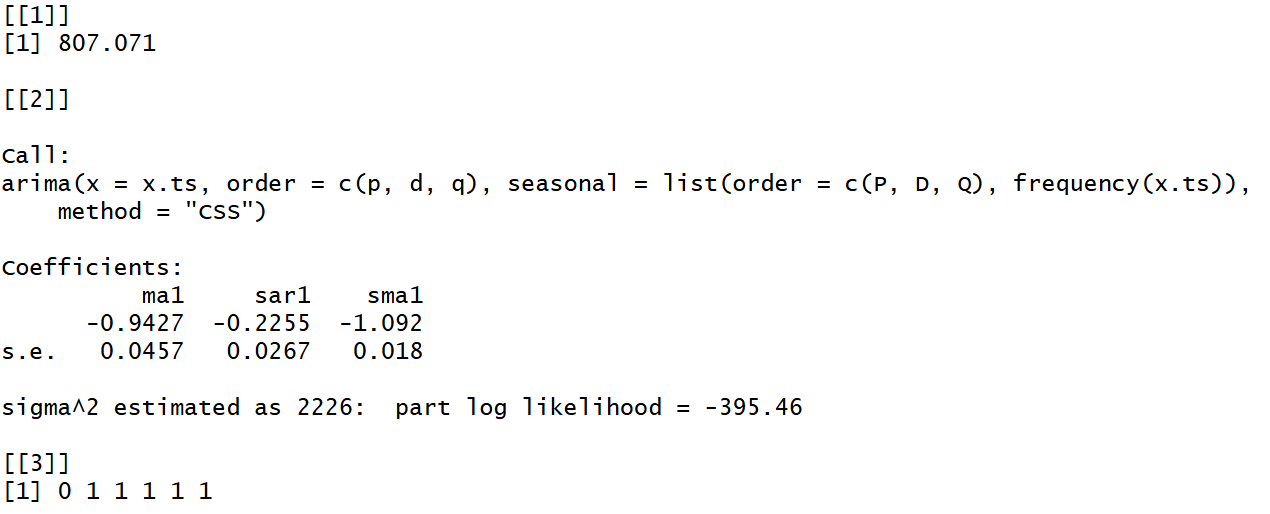
\includegraphics[width=0.75\linewidth]{fig/y2coef.png}
\end{figure}
\vspace{-0.4cm}

\begin{figure}[H]
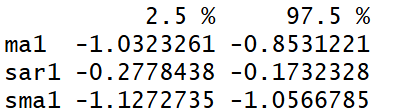
\includegraphics[width=0.25\linewidth]{fig/y2ci.png}
\end{figure}

\noindent All three coefficients are significantly different from zero, as none of the confidence intervals include zero; hence, no terms are removed. The fitted model with $\sigma^2 = 2226$ is

\vspace{-0.5cm}

\begin{align*}
x_t-x_{t-1}-x_{t-4}+x_{t-5}
&= w_t -0.9427w_{t-1}\\
&\quad -0.2255(x_{t-4}-x_{t-5})
-1.092w_{t-4}.
\end{align*}

\vspace{-0.5cm}

\begin{figure}[H]
    \centering
    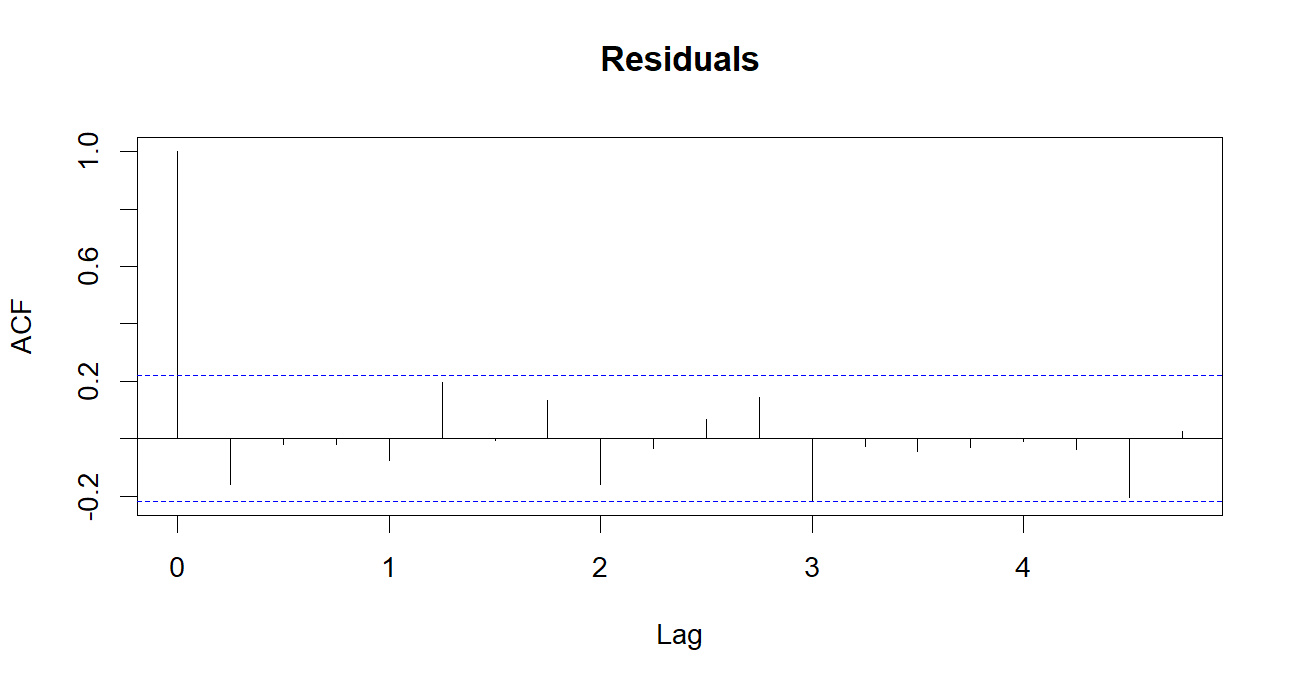
\includegraphics[width=0.75\linewidth]{fig/y2qr.png}
\end{figure}

\noindent The residual correlogram shows no significant autocorrelation, indicating white-noise behaviour and suggesting that the model adequately captures the trend and seasonal patterns in the Holiday series. The \textbf{ARIMA$(0,1,1)(1,1,1)_4$} model is therefore selected as the final specification for the Holiday series.




\subsection{Conclusion of the Two Series}

\noindent In conclusion, both Business and Holiday series were found to be non-stationary and required first and seasonal differencing before model fitting. The final selected models are ARIMA$(1,1,2)(2,1,0)_4$ for the Business series and ARIMA$(0,1,1)(1,1,1)_4$ for the Holiday series. Both models have significant coefficients and their residuals show white-noise behaviour, indicating that the models provide adequate fits for forecasting future quarterly trips.